%%%%%%%%%%%%%%%%%%%%%%%%%%%%%%%%%%%%%%%%%
% Focus Beamer Presentation
% LaTeX Template
% Version 1.0 (8/8/18)
%
% This template has been downloaded from:
% http://www.LaTeXTemplates.com
%
% Original author:
% Pasquale Africa (https://github.com/elauksap/focus-beamertheme) with modifications by 
% Vel (vel@LaTeXTemplates.com)
%
% Template license:
% GNU GPL v3.0 License
%
% Important note:
% The bibliography/references need to be compiled with bibtex.
%
%%%%%%%%%%%%%%%%%%%%%%%%%%%%%%%%%%%%%%%%%

%----------------------------------------------------------------------------------------
%	PACKAGES AND OTHER DOCUMENT CONFIGURATIONS
%----------------------------------------------------------------------------------------

\documentclass[aspectratio=1610]{beamer}
\usepackage[style=authoryear]{biblatex}
\usepackage{perpage}
\usepackage{subcaption}
\MakePerPage{footnote}
\addbibresource{example.bib}
\usepackage{xcolor}
\newcommand{\red}[1]{\textcolor{red}{#1}}
\usepackage[labelformat=empty]{caption}
\usepackage{minted}
\usepackage[Q=yes]{examplep}
\usepackage[T1]{fontenc}
\renewcommand*{\bibfont}{\normalfont\tiny}
\usepackage{makecell}

\usetheme{focus} % Use the Focus theme supplied with the template
% Add option [numbering=none] to disable the footer progress bar
% Add option [numbering=fullbar] to show the footer progress bar as always full with a slide count

% Uncomment to enable the ice-blue theme
\definecolor{main}{RGB}{0, 80, 60} % 维多利亚大学校徽的深绿色
\definecolor{background}{RGB}{255, 255, 255} % 背景纯白色

\newcommand{\vuwlogo}{%
    \begin{tikzpicture}[remember picture,overlay]
    \node[anchor=north east,yshift=3.5pt,xshift=0pt] at (current page.north east) {
\includegraphics[height=0.95cm]{Images/vuw.png}};
%    \node[anchor=north east,yshift=3.5pt,xshift=-70pt] at (current page.north east) {
\includegraphics[height=0.95cm]{Images/GECCO 2024.png}};
    \end{tikzpicture}%
}

%------------------------------------------------

\usepackage{booktabs} % Required for better table rules

%----------------------------------------------------------------------------------------
%	 TITLE SLIDE
%----------------------------------------------------------------------------------------


\title{P-Mixup: Improving Generalization Performance of Evolutionary Feature Construction with Pessimistic Vicinal Risk Minimization}

\author{
    Hengzhe Zhang, Qi Chen, Bing Xue, Wolfgang Banzhaf, Mengjie Zhang
}

\institute{Victoria University of Wellington}

\date{06/09/2024}

%------------------------------------------------

\begin{document}

%------------------------------------------------

    \begin{frame}
        \maketitle % Automatically created using the information in the commands above
    \end{frame}

    \begin{frame}{Table of Contents}
        \tableofcontents
        \vuwlogo
    \end{frame}

%----------------------------------------------------------------------------------------
%	 SECTION 1
%----------------------------------------------------------------------------------------


    \section{Background}

    \begin{frame}{Automated Feature Construction}
        \vuwlogo
        \begin{itemize}
            \item \textbf{Objective:} Construct \alert{a set of new features}, $\{\phi_1, \dots, \phi_m\}$, to \textit{enhance learning} on the dataset $\{\{x_1,y_1\}, \dots, \{x_n,y_n\}\}$ compared to learning on the original features $\{x^1, \dots, x^p\}$.
            \item \textbf{Approaches:}
            \begin{itemize}
                \item Kernel Methods: Black-box, non-parametric.
                \item Neural Networks: Black-box, gradient-based.
                \item \alert{Genetic Programming: Interpretable, gradient-free.}
            \end{itemize}
        \end{itemize}

        \begin{center}
            \begin{figure}
                \begin{subfigure}[b]{0.45\textwidth}
                    \centering
                    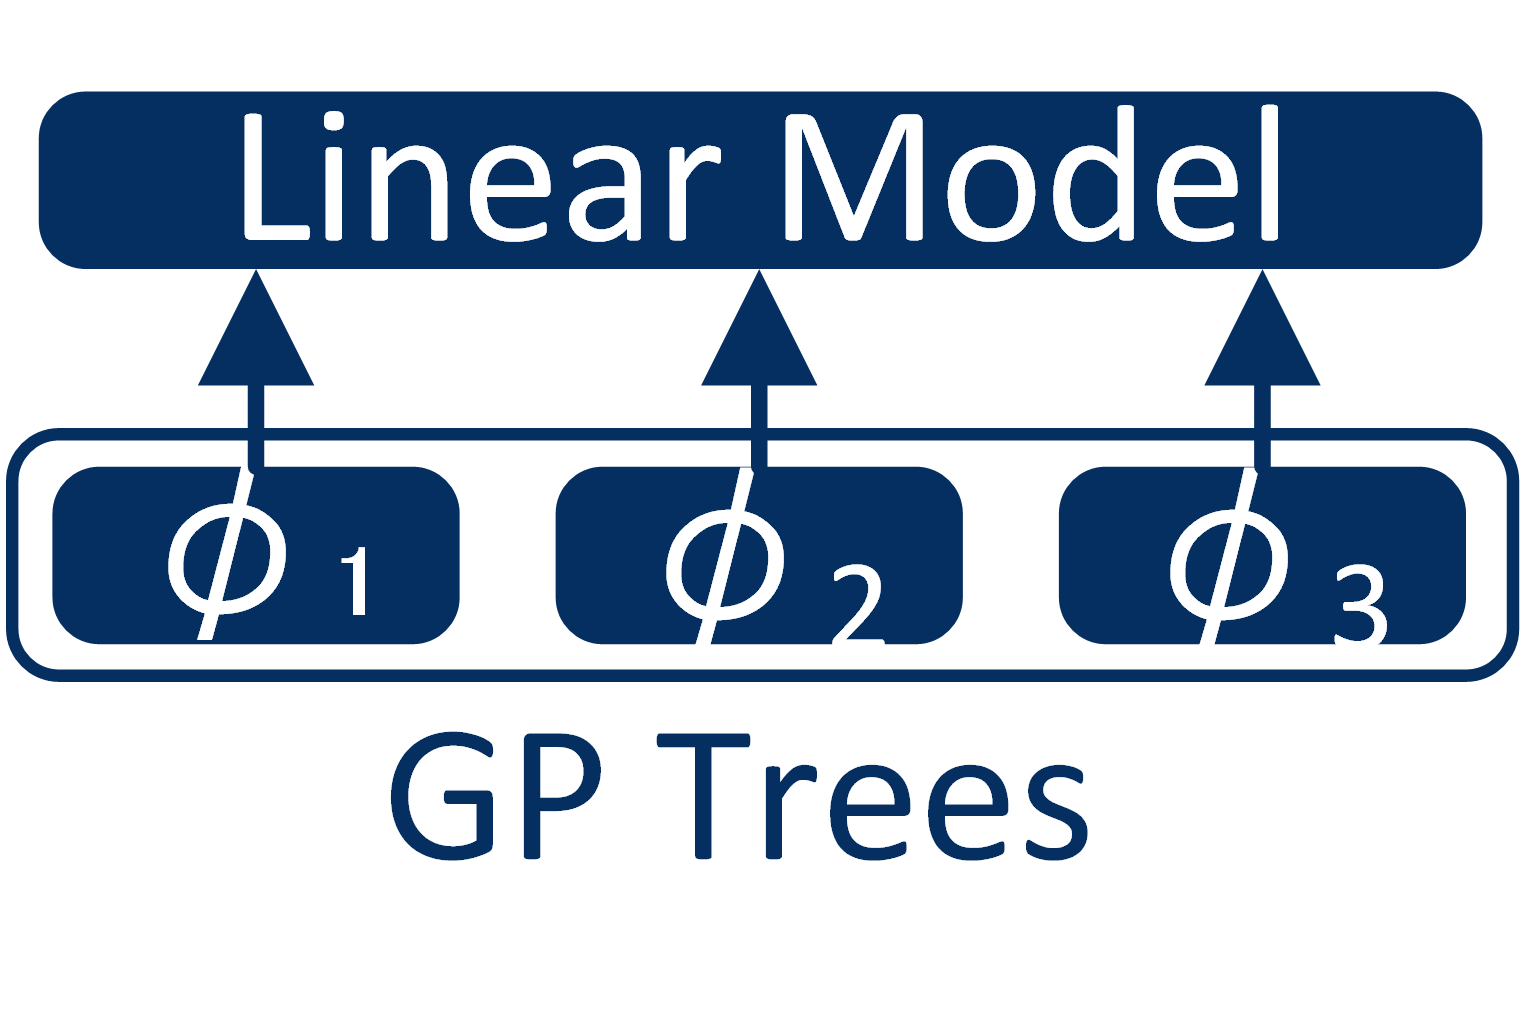
\includegraphics[width=0.6\linewidth]{Images/representation.png}
                    \caption{Feature Construction on Linear Regression}
                \end{subfigure}
                \begin{subfigure}[b]{0.45\textwidth}
                    \centering
                    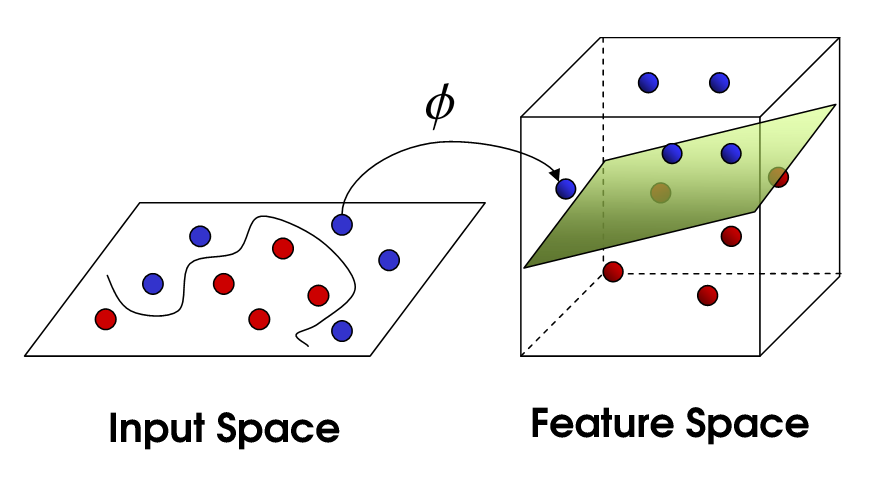
\includegraphics[width=0.75\linewidth]{Images/Kernel.png}
                    \caption{New Feature Space}
                \end{subfigure}
            \end{figure}
        \end{center}
    \end{frame}

    \begin{frame}{Overfitting}
        \vuwlogo
        \begin{itemize}
            \item \textbf{Challenge:} \alert{Overfitting} is a significant issue in evolutionary feature construction.
            \item \textbf{Phenomenon:} Overfitted models perform well on training data but poorly on unseen data.
            \item \textbf{Cause:} Models may become too complex and fit noise in the training data, especially when:
            \begin{itemize}
                \item Sample size is limited.
                \item Data contains noise.
            \end{itemize}
        \end{itemize}
        \begin{block}{Objective}
            \alert{Mitigate overfitting} to enhance generalization and robustness of constructed features.
        \end{block}
    \end{frame}


    \begin{frame}{Empirical Risk Minimization (ERM)}
        \vuwlogo
        \begin{itemize}
            \item \textbf{ERM (Empirical Risk Minimization):}
            \begin{equation}
                \mathcal{L}(f) = \frac{1}{n} \sum_{i=1}^{n} \mathcal{L}(f(x_i), y_i)
            \end{equation}
            \item \textbf{Concept:}
            \begin{itemize}
                \item \alert{ERM minimizes the average loss} over the training data.
                \item \alert{Focuses only on given data points} $(x_i, y_i)$ without considering neighbors or unseen data.
            \end{itemize}
        \end{itemize}
        \begin{figure}[!tb]
            \centering
            \includegraphics[width=0.4\linewidth]{Images/vrm.pdf}
        \end{figure}
    \end{frame}

    \begin{frame}{Vicinal Risk Minimization (VRM)}
        \vuwlogo
        \begin{itemize}
            \item \textbf{VRM (Vicinal Risk Minimization):}
            \begin{equation}
                \mathcal{VIC}(f) = \frac{1}{n} \sum_{i=1}^{n} \int \mathcal{L}(f(\mathbf{x}), y_i) dP_{x_i}(\mathbf{x})
            \end{equation}
            \item \textbf{Concept:}
            \begin{itemize}
                \item \alert{VRM incorporates vicinal samples} (neighbors of training points).
                \item It minimizes the expected loss over a \alert{distribution of neighboring samples} $P_{x_i}$ around each training point.
            \end{itemize}
        \end{itemize}
        \begin{figure}[!tb]
            \centering
            \includegraphics[width=0.4\linewidth]{Images/vrm.pdf}
        \end{figure}
    \end{frame}

    \begin{frame}{Gaussian Synthesis}
        \vuwlogo
        \begin{itemize}
            \item \textbf{Concept:}
            \begin{itemize}
                \item \alert{Gaussian Synthesis} generates vicinal samples by adding Gaussian noise to the original training data.
                \item The noise is sampled from a normal distribution $\mathcal{N}(0, \sigma^2)$, where $\sigma$ represents the standard deviation.
            \end{itemize}
            \item \textbf{Limitation:}
            \begin{itemize}
                \item \alert{Gaussian noise may create synthetic samples that do not lie on the true data manifold.}
            \end{itemize}
        \end{itemize}
        \begin{figure}[!tb]
            \centering
            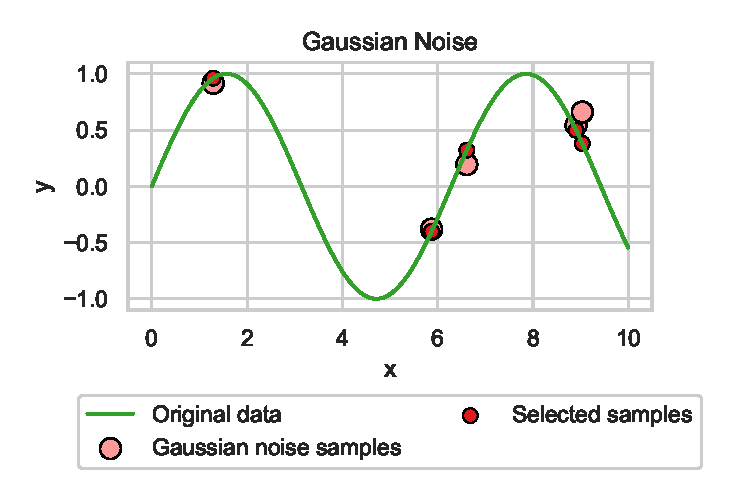
\includegraphics[width=0.4\linewidth]{Images/gaussian_noise.eps}
        \end{figure}
    \end{frame}


    \section{Method}
    \begin{frame}{MixUp Synthesis}
        \vuwlogo
        \begin{itemize}
            \item \textbf{Concept:}
            \begin{itemize}
                \item \alert{MixUp Synthesis} generates new vicinal samples by linearly combining two training samples $x_a$ and $x_b$.
                \item The formula for the synthesized sample is:
                \begin{equation}
                    x_{\text{mixup}} = \lambda \cdot x_a + (1-\lambda) \cdot x_b
                \end{equation}
                where $\lambda \in [0,1]$ is a randomly sampled mixing ratio.
            \end{itemize}
            \item \textbf{Objective:} \alert{Create synthetic samples that lie between two real data points}, helping the model generalize by learning from intermediate data.
        \end{itemize}
        \begin{figure}[!tb]
            \centering
            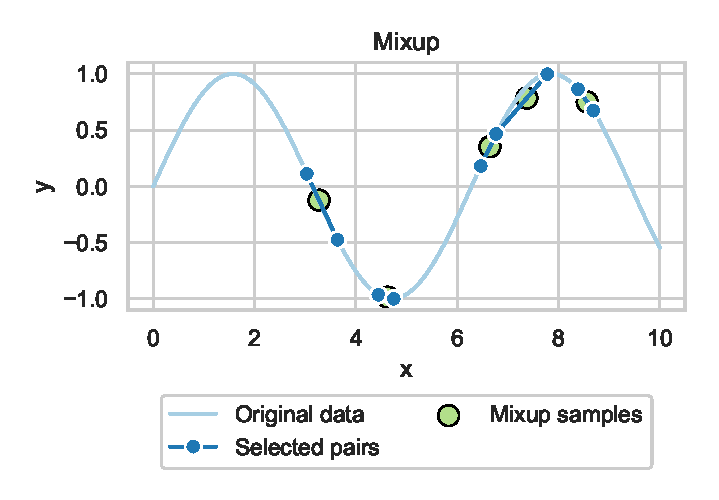
\includegraphics[width=0.4\linewidth]{Images/mixup.eps}
        \end{figure}
    \end{frame}

    \begin{frame}{Pessimistic Vicinal Risk Minimization (P-VRM)}
        \vuwlogo
        \begin{itemize}
            \item \textbf{P-VRM (Pessimistic Vicinal Risk Minimization):}
            \begin{equation}
                \mathcal{V}(f) = \frac{1}{n} \sum_{i=1}^{n} \max_{x \in \mathbb{N}(x_i)} \mathcal{L}(f(\mathbf{x}), y_i)
            \end{equation}
            \item \textbf{Concept:}
            \begin{itemize}
                \item \alert{P-VRM minimizes the worst-case loss} among the vicinal samples in the neighborhood $\mathbb{N}(x_i)$ of each training point.
                \item Focusing on the worst-case scenario, the model becomes more robust and stable, improving generalization to unseen samples.
            \end{itemize}
        \end{itemize}
        \begin{figure}[!tb]
            \centering
            \includegraphics[width=0.35\linewidth]{Images/vrm.pdf}
        \end{figure}
    \end{frame}

    \begin{frame}{Key Algorithm Components}
        \vuwlogo
        \begin{itemize}
            \item \textbf{Population Initialization:} GP trees are initialized using the ramped-half-and-half method.
            \item \textbf{Parent Selection:} Lexicase selection is used to select parents by iteratively eliminating poorly performing individuals on some instances.
            \item \textbf{Offspring Generation:} Random subtree crossover, mutation, and dynamic tree addition/deletion operators.
            \item \textbf{Objective Evaluation:}
            \begin{itemize}
                \item Vicinal data is synthesized using the \alert{mixup technique}.
                \item \alert{Pessimistic vicinal risk} and \alert{cross-validation loss} are evaluated.
            \end{itemize}
            \item \textbf{Final Model Selection:} Based on the lowest vicinal risk.
        \end{itemize}
    \end{frame}

    \begin{frame}{Pessimistic MixUp: Local Linearity Promotion}
        \vuwlogo
        \begin{itemize}
            \item \textbf{Theorem:} Pessimistic MixUp encourages local linearity around each sample $x_a \in X$ by minimizing the objective:
            \[
                \max_{\lambda, (x_b, y_b) \in \mathbb{N}(x_a)} (0.5 - |\lambda - 0.5|)^2 (y_b - y_a - \nabla f(x_a)^\top (x_b - x_a))^2
            \]
            where $\lambda \sim \text{Beta}(\alpha, \beta)$ is the MixUp ratio.
            \item The optimal gradient is:
            \[
                \nabla f(x_a) = \frac{(y_b^* - y_a)}{\|\Delta x\|^2} \Delta x
            \]
            where $\Delta x = (x_b^* - x_a)$.
        \end{itemize}
    \end{frame}

    \begin{frame}{Optimal Gradient Interpretation}
        \vuwlogo
        \begin{itemize}
            \item \textbf{The optimal gradient is:}
            \[
                \nabla f(x_a) = \frac{(y_b^* - y_a)}{\|\Delta x\|^2} \Delta x
            \]
            where \(\Delta x = (x_b^* - x_a)\).
            \item This is not \(\nabla f(x_a) = x_a^2\) or \(\nabla f(x_a) = x_a^3\). Instead, it is a constant vector.
            \item A \textbf{constant gradient} implies that the function \(f(x)\) behaves \alert{linearly} in the local region around \(x_a\).
        \end{itemize}
    \end{frame}


    \section{Experimental Settings}

    \begin{frame}{Datasets}
        \vuwlogo
        \begin{itemize}
            \item \textbf{Source:} 58 real-world datasets from the Penn Machine Learning Benchmark (PMLB).
            \item \textbf{Criteria:} Excluded synthetic datasets.
            \item \textbf{Focus:} Emphasis on real-world applicability.
        \end{itemize}
    \end{frame}

    \begin{frame}{Parameter Settings}
        \vuwlogo
        \begin{table}[!tb]
            \centering
            \caption{Parameter Settings for GP}
            \begin{tabular}{cc}%
                \begin{minipage}[t]{0.45\linewidth}
                    \scriptsize
                    \begin{tabular}{cc}
                        \toprule
                        \textbf{Parameter}      & \textbf{Value} \\
                        \midrule
                        Maximum Population Size & 200            \\
                        Number of Generations   & 100            \\
                        Crossover Rate          & 0.9            \\
                        Mutation Rate           & 0.1            \\
                        Tree Addition Rate      & 0.5            \\
                        Tree Deletion Rate      & 0.5            \\
                        Initial Tree Depth      & 0-3            \\
                        Maximum Tree Depth      & 10             \\
                        Initial Number of Trees & 1              \\
                        \bottomrule
                    \end{tabular}
                \end{minipage}
                &
                \begin{minipage}[t]{0.5\linewidth}
                    \scriptsize
                    \begin{tabular}{cc}
                        \toprule
                        \textbf{Parameter}                  & \textbf{Value}         \\
                        \midrule
                        Maximum Number of Trees             & 10                     \\
                        Elitism (Number of Individuals)     & 1                      \\
                        Bandwidth of Gaussian Kernel        & 0.5                    \\
                        $\beta$ of Beta Distribution        & 1                      \\
                        Iterations of Risk Estimation ($K$) & 10                     \\
                        Functions                           & \makecell{+, -, *, AQ, \\ Abs, Sqrt, Neg, \\ Log, Max, Min, \\ Sin, Cos, Square}                           \\
                        \bottomrule
                    \end{tabular}
                \end{minipage}
            \end{tabular}
            \label{tab:parameter_settings}%
        \end{table}
    \end{frame}

    \begin{frame}{Benchmark Methods}
        \vuwlogo
        \textbf{Compared Methods:}
        \begin{itemize}
            \item Standard GP without regularization
            \item Parsimonious Pressure (PP)
            \item Tikhonov Regularization (TK)
            \item Grand Complexity (GC)
            \item Rademacher Complexity (RC)
            \item Weighted MIC between Residuals and Variables (WCRV)
            \item Correlation between Input and Output Distances (IODC)
        \end{itemize}
    \end{frame}


    \section{Results}

    \begin{frame}{Training Performance}
        \vuwlogo
        \begin{itemize}
            \item \alert{Training $R^2$: Standard GP is the best}.
        \end{itemize}

        \begin{table}[!tb]
            \centering
            \caption{Statistical comparison of training $R^2$ scores.}
            \scriptsize
            \begin{tabular}{ccccc}%
                \toprule%
                & \textbf{VRM}             & \textbf{PP}              & \textbf{RC}              & \textbf{GC}             \\%
                \midrule%
                \textbf{P-VRM} & 0(+)/14($\sim$)/44({-})  & 28(+)/17($\sim$)/13({-}) & 56(+)/2($\sim$)/0({-})& 46(+)/10($\sim$)/2({-})\\%
                \textbf{VRM}   & ---                      & 48(+)/10($\sim$)/0({-})  & 58(+)/0($\sim$)/0({-})   & 56(+)/2($\sim$)/0({-})  \\%
                \textbf{PP}    & ---                      & ---                      & 58(+)/0($\sim$)/0({-})   & 46(+)/12($\sim$)/0({-}) \\%
                \textbf{RC}    & ---                      & ---                      & ---                      & 1(+)/4($\sim$)/53({-})  \\%
                \midrule%
                & \textbf{IODC}            & \textbf{TK}              & \textbf{WCRV}            & \textbf{Standard GP}    \\%
                \midrule%
                \textbf{P-VRM} & 37(+)/15($\sim$)/6({-})  & 36(+)/15($\sim$)/7({-})  & 39(+)/13($\sim$)/6({-})& 1(+)/13($\sim$)/44({-})\\%
                \textbf{VRM}   & 53(+)/5($\sim$)/0({-})   & 53(+)/4($\sim$)/1({-})   & 48(+)/8($\sim$)/2({-})& 2(+)/38($\sim$)/18({-})\\%
                \textbf{PP}    & 29(+)/23($\sim$)/6({-})  & 32(+)/20($\sim$)/6({-})  & 38(+)/15($\sim$)/5({-})& 0(+)/3($\sim$)/55({-})\\%
                \textbf{RC}    & 1(+)/4($\sim$)/53({-})   & 0(+)/1($\sim$)/57({-})   & 2(+)/9($\sim$)/47({-})& 0(+)/0($\sim$)/58({-})\\%
                \textbf{GC}    & 12(+)/27($\sim$)/19({-}) & 11(+)/26($\sim$)/21({-}) & 23(+)/25($\sim$)/10({-})& 0(+)/1($\sim$)/57({-})\\%
                \textbf{IODC}  & ---                      & 16(+)/19($\sim$)/23({-}) & 27(+)/19($\sim$)/12({-}) & 0(+)/0($\sim$)/58({-})  \\%
                \textbf{TK}    & ---                      & ---                      & 31(+)/12($\sim$)/15({-}) & 0(+)/4($\sim$)/54({-})  \\%
                \textbf{WCRV}  & ---                      & ---                      & ---                      & 0(+)/2($\sim$)/56({-})  \\%
                \bottomrule%
            \end{tabular}%
        \end{table}
    \end{frame}

    \begin{frame}{Test Performance}
        \vuwlogo
        \begin{itemize}
            \item \alert{Test $R^2$: P-VRM significantly improves generalization compared to standard GP and other overfitting control methods.}
            \item P-VRM outperforms VRM, indicating the effectiveness of pessimistic vicinal risk minimization.
        \end{itemize}

        \begin{table}[!tb]
            \centering
%            \caption{Statistical comparison of test $R^2$ scores.}
            \scriptsize
            \begin{tabular}{ccccc}%
                \toprule%
                & \textbf{VRM}            & \textbf{PP}              & \textbf{RC}              & \textbf{GC}              \\%
                \midrule%
                \textbf{P-VRM} & 22(+)/29($\sim$)/7({-}) & 22(+)/31($\sim$)/5({-})  & 46(+)/10($\sim$)/2({-})& 23(+)/32($\sim$)/3({-})\\%
                \textbf{VRM}   & ---                     & 11(+)/38($\sim$)/9({-})  & 38(+)/10($\sim$)/10({-}) & 16(+)/29($\sim$)/13({-}) \\%
                \textbf{PP}    & ---                     & ---                      & 38(+)/13($\sim$)/7({-})  & 15(+)/34($\sim$)/9({-})  \\%
                \textbf{RC}    & ---                     & ---                      & ---                      & 5(+)/10($\sim$)/43({-})  \\%
                \midrule%
                & \textbf{IODC}           & \textbf{TK}              & \textbf{WCRV}            & \textbf{Standard GP}     \\%
                \midrule%
                \textbf{P-VRM} & 31(+)/24($\sim$)/3({-}) & 44(+)/12($\sim$)/2({-})  & 38(+)/18($\sim$)/2({-})& 31(+)/21($\sim$)/6({-})\\%
                \textbf{VRM}   & 24(+)/25($\sim$)/9({-}) & 28(+)/29($\sim$)/1({-})  & 27(+)/23($\sim$)/8({-})& 22(+)/34($\sim$)/2({-})\\%
                \textbf{PP}    & 23(+)/29($\sim$)/6({-}) & 25(+)/31($\sim$)/2({-})  & 26(+)/26($\sim$)/6({-})& 25(+)/25($\sim$)/8({-})\\%
                \textbf{RC}    & 5(+)/21($\sim$)/32({-}) & 5(+)/20($\sim$)/33({-})  & 11(+)/17($\sim$)/30({-})& 13(+)/14($\sim$)/31({-})\\%
                \textbf{GC}    & 25(+)/26($\sim$)/7({-}) & 23(+)/33($\sim$)/2({-})  & 25(+)/30($\sim$)/3({-})& 24(+)/21($\sim$)/13({-})\\%
                \textbf{IODC}  & ---                     & 19(+)/24($\sim$)/15({-}) & 15(+)/30($\sim$)/13({-}) & 21(+)/16($\sim$)/21({-}) \\%
                \textbf{TK}    & ---                     & ---                      & 11(+)/33($\sim$)/14({-}) & 10(+)/27($\sim$)/21({-}) \\%
                \textbf{WCRV}  & ---                     & ---                      & ---                      & 17(+)/22($\sim$)/19({-}) \\%
                \bottomrule%
            \end{tabular}%
        \end{table}
    \end{frame}
    \begin{frame}{Training Performance}
        \vuwlogo
        \begin{itemize}
            \item \textbf{Correlation between training and test $R^2$ scores:} \alert{P-VRM method effectively controls overfitting}.
        \end{itemize}

        \begin{figure}[!tb]
            \centering
            \includegraphics[width=0.5\linewidth]{Images/n_gen_train_test_plot_iteration.pdf}
            \caption{Evolutionary plots of the \textit{training and test $R^2$ scores} for VR.}
            \label{fig: Training Test Plot}
        \end{figure}
    \end{frame}
    \begin{frame}{Tree Size}
        \vuwlogo
        \begin{itemize}
            \item \textbf{Tree sizes:} P-VRM does not significantly reduce tree size compared to standard GP.
        \end{itemize}

        \begin{figure}[tb]
            \centering
            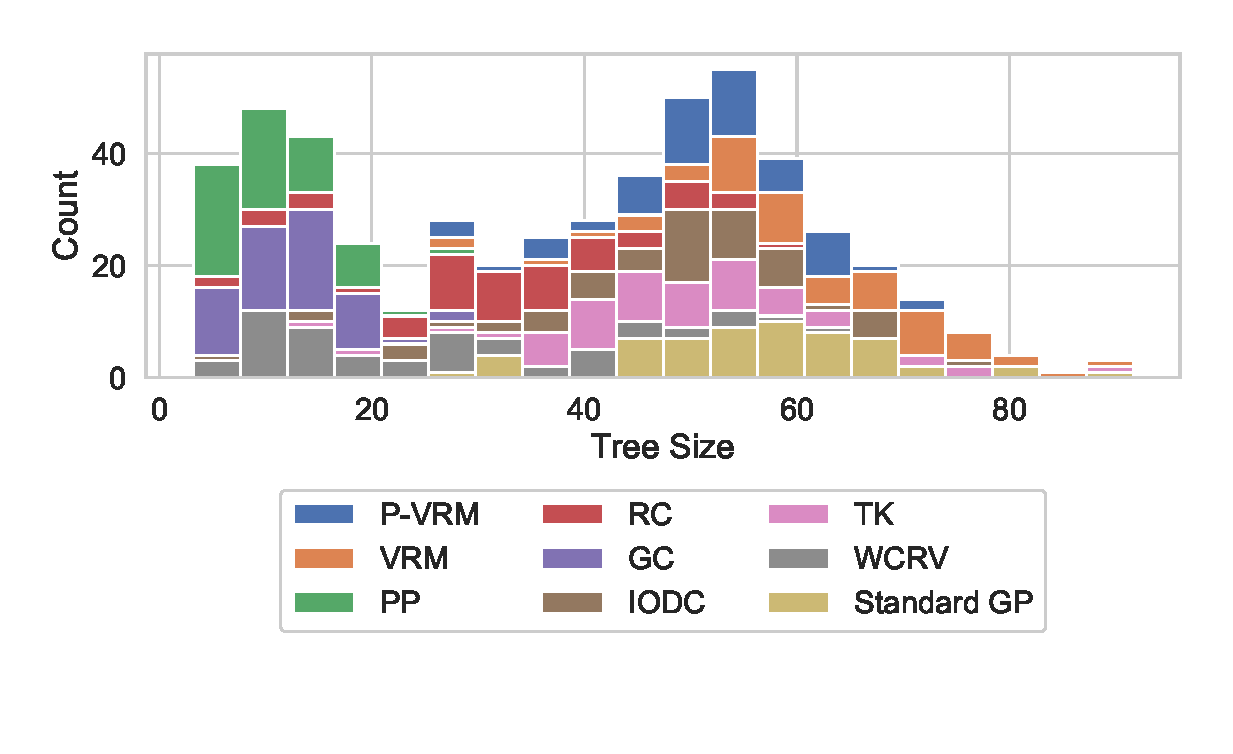
\includegraphics[width=0.65\linewidth]{Images/SAM_Size_sum_complexity.eps}
            \caption{Distribution of tree sizes across methods.}
            \label{fig: Complexity}
        \end{figure}
    \end{frame}

    \begin{frame}{Training Time}
        \vuwlogo
        \begin{itemize}
            \item \textbf{Training Time:} P-VRM method is computationally more intensive.
        \end{itemize}

        \begin{figure}[tb]
            \centering
            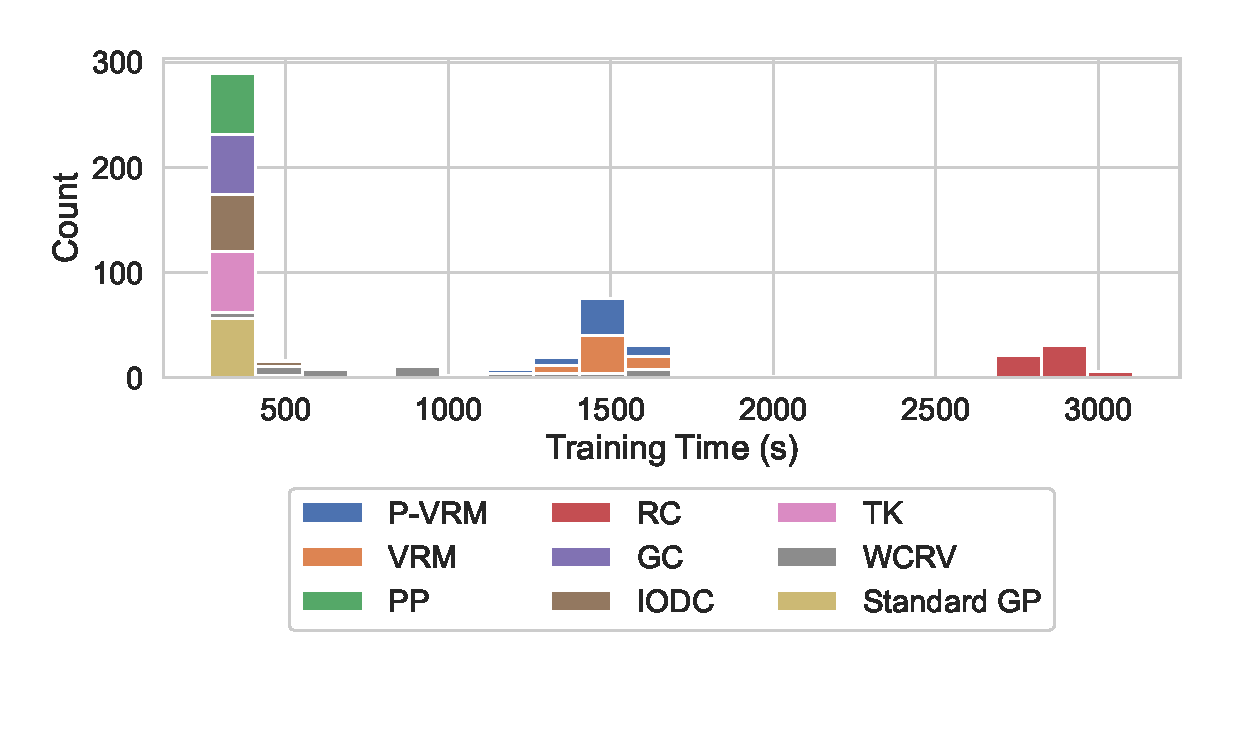
\includegraphics[width=0.65\linewidth]{Images/SAM_Time_cost_time.eps}
            \caption{Distribution of training time (seconds) across methods.}
            \label{fig: Training Time}
        \end{figure}
    \end{frame}

    \begin{frame}{Further Analysis of P-VRM}
        \begin{itemize}
            \item \textbf{Key Questions:}
            \begin{itemize}
                \item Is MixUp better than Gaussian perturbation for generating vicinal samples?
            \end{itemize}

            \item \textbf{MixUp vs. Gaussian Noise:}
            \begin{itemize}
                \item P-VRM outperforms P-GVRM on 23 datasets, worse on only 8.
                \item MixUp better aligns with the data manifold than Gaussian noise.
            \end{itemize}
            \begin{table}[!h]
                \centering
                \scriptsize
                \caption{$R^2$ Score Comparison}
                \begin{tabular}{cccc}%
                    \toprule%
                    & \textbf{P-GVRM}         & \textbf{GVRM}           \\%
                    \midrule%
                    \textbf{P-VRM}  & 23(+)/27($\sim$)/8({-}) & 30(+)/21($\sim$)/7({-}) \\%
                    \textbf{P-GVRM} & ---                     & 22(+)/34($\sim$)/2({-}) \\%
                    \bottomrule%
                \end{tabular}%
            \end{table}
        \end{itemize}
    \end{frame}

    \section{Conclusions}
    \begin{frame}{Conclusions}
        \vuwlogo
        \begin{block}{\centering Key Takeaways}
            \begin{itemize}
                \item \textbf{P-VRM} minimizes worst-case vicinal risks for improved robustness.
                \item \textbf{MixUp-based vicinal samples} help the model generalize between real data points.
                \item \textbf{Empirical results:} P-VRM reduces overfitting and outperforms traditional methods.
            \end{itemize}
        \end{block}
    \end{frame}


% %------------------------------------------------

    \begin{frame}[focus]
        Thanks for listening!\\
        {
            \footnotesize
            Email: Hengzhe.zhang@ecs.vuw.ac.nz\\
            GitHub Project: https://github.com/hengzhe-zhang/EvolutionaryForest
        }
    \end{frame}

%----------------------------------------------------------------------------------------
%	 CLOSING/SUPPLEMENTARY SLIDES
%----------------------------------------------------------------------------------------

    \appendix

% \begin{frame}{References}
% 	\nocite{*} % Display all references regardless of if they were cited
% \bibliography{example.bib}
% \bibliographystyle{plain}
% \end{frame}

%------------------------------------------------

% \begin{frame}{Backup Slide}
% 	This is a backup slide, useful to include additional materials to answer questions from the audience.
% 	\vfill
% 	The package \texttt{appendixnumberbeamer} is used to refrain from numbering appendix slides.
% \end{frame}

%----------------------------------------------------------------------------------------

\end{document}
